\documentclass[12pt, a4paper]{article}

% ── Kódování a jazyk ──
\usepackage[utf8]{inputenc}
\usepackage[T1]{fontenc}
\usepackage[czech]{babel}

% ── Typografie a layout ──
\usepackage{lmodern}
\usepackage[margin=2.5cm]{geometry}
\usepackage{setspace}
\onehalfspacing
\emergencystretch=2em

% ── Matematika, tabulky, obrázky ──
\usepackage{amsmath}
\usepackage{amssymb}
\usepackage{booktabs}
\usepackage{graphicx}
\usepackage{float}
\usepackage{caption}
\usepackage{subcaption}

% ── Zalamování dlouhých texttt ──
\newcommand{\modelname}{\texttt{paraphrase-\allowbreak{}multilingual-\allowbreak{}MiniLM-\allowbreak{}L12-\allowbreak{}v2}}

% ── Odkazy ──
\usepackage{xcolor}
\usepackage[colorlinks=true, linkcolor=blue!60!black, citecolor=blue!60!black, urlcolor=blue!60!black]{hyperref}

% ══════════════════════════════════════════════════════════════════════
\title{%
  Political Discourse Topology:\\[4pt]
  Kvantitativní perspektiva sémantického prostoru\\
  předvolebních debat 2025%
}

\author{%
  {\normalsize Katedra obecné lingvistiky, Univerzita Palackého v~Olomouci}\\[2pt]
  {\normalsize Předmět: KRAD — Kvantitativní analýza diskurzu}%
}

\date{Březen 2026}

\begin{document}
\maketitle

% ══════════════════════════════════════════════════════════════════════
\begin{abstract}
Předkládaná studie navrhuje a~aplikuje kvantitativní pipeline pro analýzu
politického diskurzu na korpusu 7\,715 promluv z~předvolebních debat České
televize (podzim~2025). Metodologický rámec integruje sentence embeddingy
(model \modelname{}), redukci dimenzí
algoritmem UMAP, lexikální metriky (Type-Token Ratio, Maas index) a~volitelné
obohacení promluv pomocí velkého jazykového modelu (sentiment, agresivita,
rétorickéé rámce). Výsledky vizualizované prostřednictvím sémantické mapy,
bubble chartu rétorického profilu a~heatmapy tematické dominance ukazují
výraznou konvergenci středových stran v~sémantickém prostoru, odlišnou
syntaktickou komplexitu Pirátů a~specifické tematické strategie
protisystémových subjektů. Navržená metoda demonstruje potenciál komputačních
přístupů pro obecnou lingvistiku a~kritickou analýzu diskurzu.
\end{abstract}

\bigskip
\noindent\textbf{Klíčová slova:}
politický diskurz, sentence embeddings, UMAP, lexikální diverzita,
Maas index, kvantitativní lingvistika, NLP, předvolební debaty

\newpage
\tableofcontents
\newpage

% ══════════════════════════════════════════════════════════════════════
\section{Úvod}
\label{sec:uvod}

Předvolební kampaň před parlamentními volbami v~říjnu 2025 představovala
v~českém politickém prostředí událost s~vysokou diskurzivní dynamikou.
Televizní debaty České televize, vysílané od září do října~2025, poskytly
systematický a~veřejně přístupný zdroj politických promluv pokrývající
široké spektrum témat — od ekonomiky přes vzdělávání po zahraniční politiku.
Tento materiál tak vytváří vhodný korpus pro kvantitativní analýzu
politického diskurzu.

Kritická analýza diskurzu (CDA), jak ji rozpracovali
Fairclough~(1995) a~van Dijk~(2001), byla tradičně kvalitativní
disciplínou, založenou na interpretativní práci výzkumníka s~textem.
S~rozvojem metod zpracování přirozeného jazyka (NLP) a~zejména
s~příchodem kontextuálních jazykových modelů se však otevírá prostor
pro komplementární kvantitativní přístupy, které umožňují zpracovat
rozsáhlé korpusy a~identifikovat vzorce nepozorovatelné manuální
analýzou.

Předkládaná studie si klade za cíl navrhnout a~aplikovat reprodukovatelnou
analytickou pipeline — nazvanou \textbf{Political Discourse Topology (PDT)}
— která transformuje surové textové přepisy debat na strukturované
sémantické, lexikální a~rétorické reprezentace. Konkrétně jsou formulovány
tři výzkumné otázky:

\begin{enumerate}
  \item Jak se liší sémantický prostor projevů jednotlivých politických
        stran, měřeno prostřednictvím shluků ve dvourozměrné UMAP projekci
        sentence embeddingů?
  \item Jaká je lexikální rozmanitost a~syntaktická komplexita vyjadřování
        napříč stranami, kvantifikovaná pomocí TTR a~Maas indexu?
  \item Jaké tematické a~rétorické strategie strany využívají v~kontextu
        ekonomické debaty?
\end{enumerate}

% ══════════════════════════════════════════════════════════════════════
\section{Data}
\label{sec:data}

Analyzovaný korpus tvoří přepisy debat České televize
z~předvolebního období (září--říjen~2025). Základní parametry
datového souboru shrnuje tabulka~\ref{tab:dataset}.

\begin{table}[H]
  \centering
  \caption{Přehled analyzovaného korpusu}
  \label{tab:dataset}
  \begin{tabular}{ll}
    \toprule
    \textbf{Parametr}        & \textbf{Hodnota} \\
    \midrule
    Počet promluv (speech acts)   & 7\,715 \\
    Počet politických subjektů    & 8 stran + moderátor \\
    Počet unikátních mluvčích     & 115 \\
    Počet tematických bloků       & 18 \\
    Kódování zdrojového souboru   & UTF-8 \\
    \bottomrule
  \end{tabular}
\end{table}

V~korpusu je zastoupeno osm politických subjektů: ANO, SPOLU, Piráti, STAN,
SPD, Stačilo!, Motoristé sobě a~Přísaha. Tematické bloky pokrývají oblast
ekonomiky, dopravy, zdravotnictví, průmyslu, vzdělávání, vztahů s~EU,
justice, životního prostředí, společenských výzev, digitalizace, zahraniční
politiky, bezpečnosti a~obrany, jakož i~několik přímých duelů mezi
kandidáty. Promluvy moderátorů (celkem 3\,155) jsou v~analýze zachovány jako
referenční kategorie, neboť jejich diskurzivní profil (krátké, lexikálně
diverzní výroky) poskytuje užitečný kontrast.

\begin{table}[H]
  \centering
  \caption{Počet promluv a~celkový rozsah projevů dle politického subjektu}
  \label{tab:parties}
  \begin{tabular}{lrrr}
    \toprule
    \textbf{Strana / Role} & \textbf{Počet promluv} & \textbf{Celkem slov}
      & \textbf{Počet mluvčích} \\
    \midrule
    moderátor  & 3\,155 & 70\,541 & 14 \\
    SPOLU      & 840    & 39\,055 & 13 \\
    ANO        & 721    & 38\,639 & 12 \\
    SPD        & 579    & 29\,300 & 13 \\
    Motoristé  & 546    & 27\,466 & 12 \\
    Stačilo!   & 534    & 26\,782 & 13 \\
    Přísaha    & 491    & 24\,773 & 12 \\
    STAN       & 448    & 24\,875 & 13 \\
    Piráti     & 401    & 27\,308 & 13 \\
    \bottomrule
  \end{tabular}
\end{table}

% ══════════════════════════════════════════════════════════════════════
\section{Metodologie}
\label{sec:metodologie}

Analytická pipeline PDT sestává ze šesti fází, z~nichž pátá (LLM obohacení)
je volitelná. Každá fáze implementuje princip idempotence — kontroluje
existenci výstupního souboru a~shodu počtu řádků, čímž je zajištěna
reprodukovatelnost i~efektivita opakovaných běhů.

\subsection{Fáze~1: Parsování přepisu}
\label{sec:parsing}

Surový textový přepis je transformován na strukturovaný tabulkový formát
(CSV) pomocí regulárního výrazu, který rozpoznává hlavičku promluvy ve
formátu:

\begin{verbatim}
Jméno Příjmení (Strana) [HH:MM:SS](Téma): Text promluvy
\end{verbatim}

Pokračovací řádky (bez hlavičky) jsou připojeny k~předchozí promluvě.
Pro každou promluvu jsou vypočteny odvozené atributy: časová značka
v~sekundách, počet slov, počet vět (detekce koncových interpunkčních znaků)
a~průměrná délka věty ve slovech.

\subsection{Fáze~2: Lexikální metriky}
\label{sec:lexical}

Pro kvantifikaci lexikální diverzity jsou použity dvě komplementární míry:

\paragraph{Type-Token Ratio (TTR).}
Poměr počtu unikátních slovních typů~$V$ k~celkovému počtu tokenů~$N$:
\begin{equation}
  \mathrm{TTR} = \frac{|V|}{|N|}
  \label{eq:ttr}
\end{equation}
Hodnota blízká~1{,}0 indikuje vysokou lexikální variabilitu; hodnota blízká~0
naopak signalizuje vysokou míru opakování.

\paragraph{Maas index (Maas, 1972).}
Logaritmická transformace, která tlumí závislost na délce textu:
\begin{equation}
  a^2 = \frac{\log N - \log V}{(\log N)^2}
  \label{eq:maas}
\end{equation}
Nižší hodnota $a^2$ indikuje vyšší lexikální bohatství. Tato míra je
vhodnější pro komparativní analýzu promluv různých délek než prostý TTR.

Tokenizace je záměrně implementována jazykově agnostickým způsobem
(převod na malá písmena, segmentace na mezerách), čímž je zajištěna
transparentnost a~nezávislost na externích morfologických nástrojích.

\subsection{Fáze~3: Sentence embeddingy}
\label{sec:embeddings}

Každá promluva je zakódována do hustého vektorového prostoru pomocí
modelu \modelname{} z~knihovny Sentence Transformers
(Reimers a~Gurevych, 2019). Jedná se o~dvanáctivrstvý
multilinguální model založený na architektuře MiniLM, trénovaný na
parafrázových párech ve více než~50 jazycích včetně češtiny. Výstupní
dimenze embeddingu je~384.

Model produkuje pro každou promluvu vektor $\mathbf{e}_i \in \mathbb{R}^{384}$,
kde sémanticky podobné promluvy mají vysokou kosinovou podobnost. Celkem bylo
zakódováno 7\,715~promluv s~velikostí dávky~64.

\subsection{Fáze~4: Redukce dimenzí}
\label{sec:umap}

Pro vizualizaci 384-dimenzionálního embeddingového prostoru ve~dvou dimenzích
byl použit algoritmus UMAP (Uniform Manifold Approximation and Projection;
McInnes et al., 2018). UMAP zachovává jak lokální, tak globální topologickou
strukturu dat, čímž poskytuje věrohodnější vizuální reprezentaci sémantických
shluků než lineární metoda PCA. Parametry redukce: \texttt{n\_components=2},
\texttt{random\_state=42}.

Jako záložní metoda je implementována PCA ze~knihovny scikit-learn, která se
automaticky aktivuje v~prostředí bez nainstalovaného balíčku
\texttt{umap-learn}.

Pro každou politickou stranu je dále vypočten \textbf{centroid} — průměrný
embeddingový vektor všech promluv dané strany v~plném 384D prostoru.
Mezistraná kosinová vzdálenost centroidů slouží jako míra celkové sémantické
odlišnosti rétorických pozic.

\subsection{Fáze~5: LLM anotace (volitelná)}
\label{sec:enrichment}

Promluvy mohou být volitelně obohaceny o~automaticky generované anotace
pomocí modelu Claude (Anthropic API). Pro každou promluvu jsou generovány
tři tagy: \textit{sentiment} (plovoucí hodnota na škále $-1{,}0$ až~$1{,}0$),
\textit{agresivita} (celočíselná škála~0--5) a~\textit{dominantní rétorický
rámec} (kategoriální proměnná: Economic threat, National sovereignty,
Social justice, Fiscal responsibility, EU~scepticism, Party attack,
Neutral/factual).

Zpracování probíhá v~dávkách po~20~promluvách s~automatickým checkpointingem
po každé dávce, čímž je umožněno přerušení a~obnovení procesu.

\subsection{Fáze~6: Vizualizace}
\label{sec:viz}

Na základě vypočtených metrik a~embeddingů jsou generovány tři vizualizace:
sémantická mapa (scatter plot UMAP projekce), bubble chart rétorického
profilu a~heatmapa tematické dominance. Technické parametry vizualizací
jsou popsány v~sekci~\ref{sec:vysledky}.

% ══════════════════════════════════════════════════════════════════════
\section{Výsledky}
\label{sec:vysledky}

\subsection{Sémantická mapa politického diskurzu}
\label{sec:semantic_map}

Obrázek~\ref{fig:semantic_map} zobrazuje dvourozměrnou UMAP projekci
sentence embeddingů všech 7\,715~promluv. Každý bod představuje jednu
promluvu, barva kóduje stranickou příslušnost; hvězdičky označují
2D~centroidy stran.

\begin{figure}[H]
  \centering
  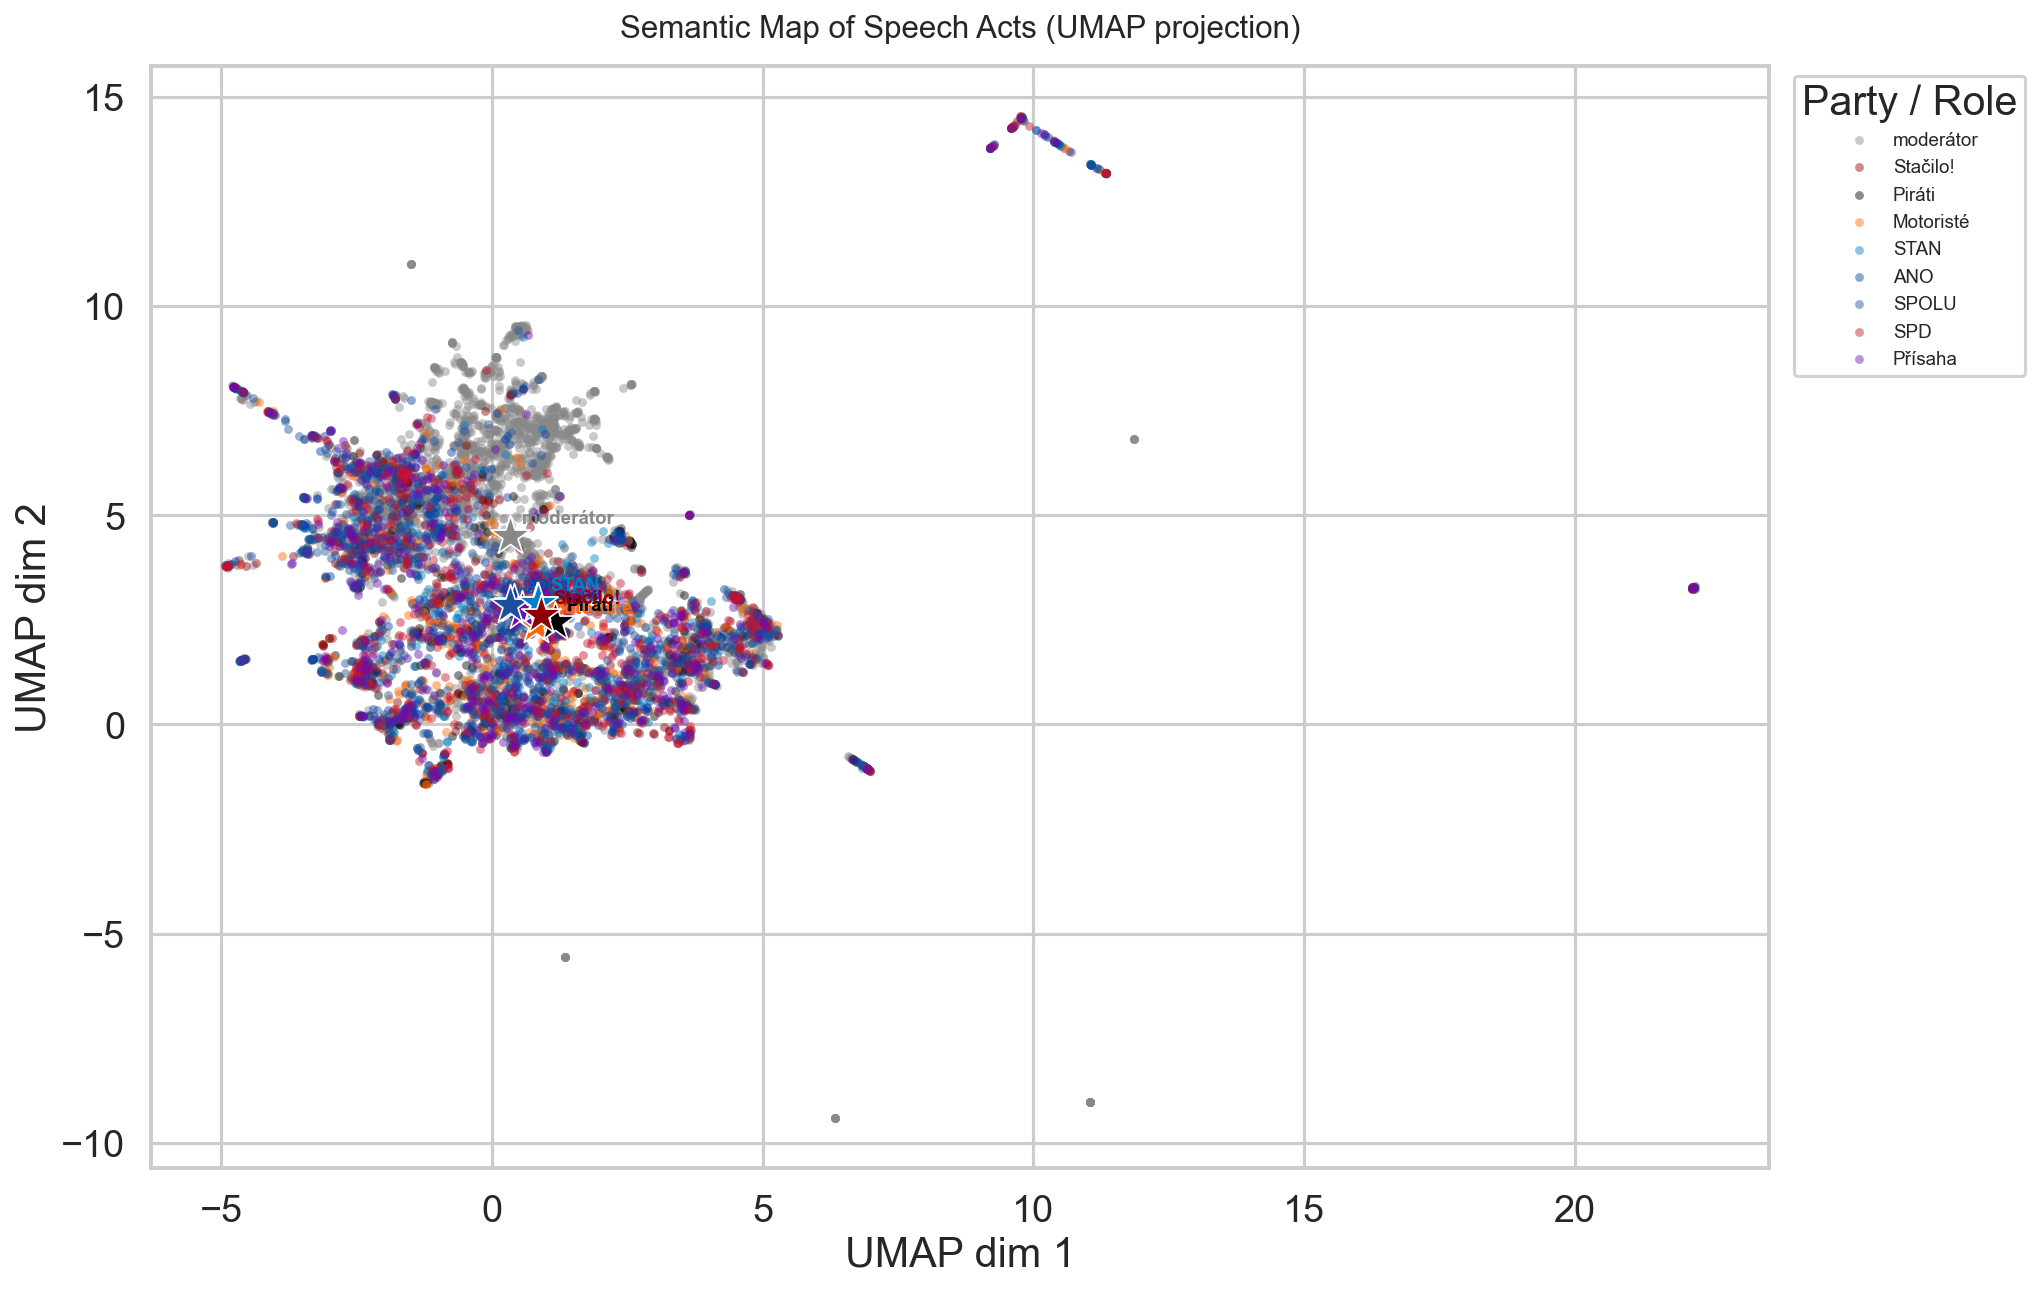
\includegraphics[width=\textwidth]{results/semantic_map.png}
  \caption{Sémantická mapa promluv (UMAP projekce). Každý bod odpovídá
  jedné promluvě, barva indikuje stranickou příslušnost. Hvězdičky
  označují centroidy stran v~2D prostoru.}
  \label{fig:semantic_map}
\end{figure}

Z~vizualizace lze identifikovat několik klíčových vzorců:

\begin{enumerate}
  \item \textbf{Centrální sémantický shluk.} Většina promluv všech
  parlamentních stran se koncentruje v~jednom dominantním shluku v~levé
  části projekce (přibližně $\mathrm{dim}_0 \in [-5, 5]$,
  $\mathrm{dim}_1 \in [0, 8]$). Tato konvergence naznačuje, že politický
  diskurz v~ekonomickém tématu sdílí značnou část sémantického prostoru
  napříč ideologickým spektrem.

  \item \textbf{Centroidy stran.} Centroidy středových a~systémových
  stran (ANO, SPOLU, STAN, Piráti) se nacházejí v~těsné blízkosti
  centra hlavního shluku, zatímco centroidy některých menších subjektů
  vykazují mírný posun. Moderátor se nachází rovněž v~blízkosti
  centrálního shluku, což odpovídá jeho tematicky neutrální,
  organizační roli.

  \item \textbf{Okrajové shluky.} V~pravé a~horní části projekce lze
  pozorovat separované menší shluky ($\mathrm{dim}_0 > 10$), které
  představují sémanticky odlišné typy promluv — pravděpodobně
  procedurální výroky, emotivní prohlášení nebo specifické duelové
  formáty. Tyto okrajové body jsou zastoupeny napříč stranami.
\end{enumerate}

\subsection{Rétorický profil: Lexikální diverzita a~syntaktická komplexita}
\label{sec:entropy}

Obrázek~\ref{fig:entropy} zobrazuje bubble chart, kde osa~$x$ reprezentuje
průměrnou lexikální diverzitu (TTR), osa~$y$ průměrnou délku věty ve~slovech
a~velikost bubliny odpovídá míře agresivity (pokud jsou dostupné LLM tagy).

\begin{figure}[H]
  \centering
  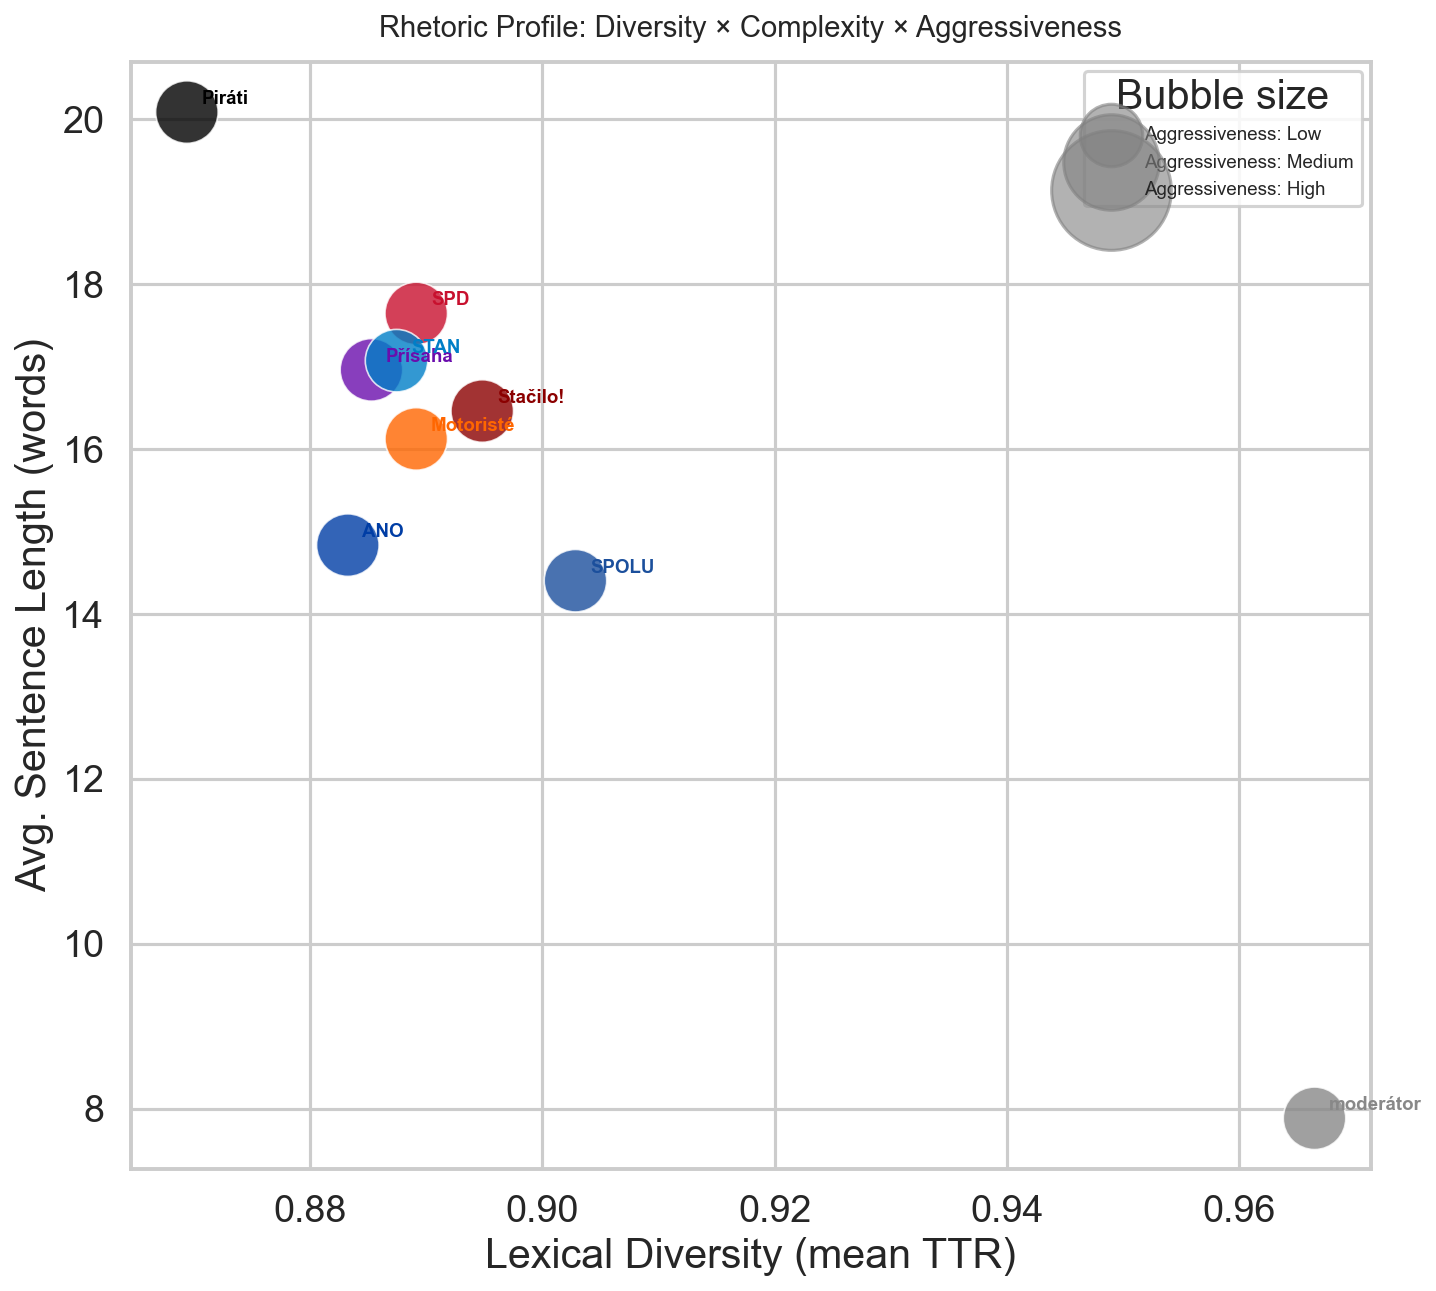
\includegraphics[width=0.9\textwidth]{results/entropy_complexity.png}
  \caption{Rétorický profil stran: lexikální diverzita (TTR) na ose~$x$,
  průměrná délka věty na ose~$y$. Velikost bubliny odpovídá míře
  agresivity.}
  \label{fig:entropy}
\end{figure}

Kvantitativní hodnoty lexikálních metrik shrnuje tabulka~\ref{tab:lexical}.

\begin{table}[H]
  \centering
  \caption{Lexikální metriky dle politického subjektu (seřazeno dle TTR)}
  \label{tab:lexical}
  \begin{tabular}{lrrrr}
    \toprule
    \textbf{Strana / Role} & \textbf{$\overline{\mathrm{TTR}}$} & \textbf{$\overline{a^2}$ (Maas)}
      & \textbf{$\overline{\ell}$ (slov/věta)} & \textbf{Celkem slov} \\
    \midrule
    moderátor  & 0{,}967 & 0{,}005 &  7{,}9 & 70\,541 \\
    SPOLU      & 0{,}903 & 0{,}008 & 14{,}4 & 39\,055 \\
    Stačilo!   & 0{,}895 & 0{,}008 & 16{,}5 & 26\,782 \\
    SPD        & 0{,}889 & 0{,}009 & 17{,}6 & 29\,300 \\
    Motoristé  & 0{,}889 & 0{,}009 & 16{,}1 & 27\,466 \\
    STAN       & 0{,}887 & 0{,}008 & 17{,}1 & 24\,875 \\
    Přísaha    & 0{,}885 & 0{,}009 & 17{,}0 & 24\,773 \\
    ANO        & 0{,}883 & 0{,}010 & 14{,}8 & 38\,639 \\
    Piráti     & 0{,}869 & 0{,}008 & 20{,}1 & 27\,308 \\
    \bottomrule
  \end{tabular}
\end{table}

Z~dat vyplývají následující pozorování:

\begin{enumerate}
  \item \textbf{Piráti jako outlier syntaktické komplexity.} Piráti
  vykazují nejvyšší průměrnou délku věty (20{,}1~slov) při současně
  nejnižším TTR mezi politickými stranami (0{,}869). Tato kombinace
  naznačuje tendenci k~delším, argumentačně strukturovaným souvětím
  s~vyšší mírou lexikální repetice. Jde o~diskurzivní styl
  charakteristický pro expertní, technicistní rétoriku.

  \item \textbf{ANO a~SPOLU: kompaktní vyjadřování.} Obě strany
  s~nejvyšším celkovým počtem slov vykazují nižší průměrnou délku věty
  (ANO:~14{,}8; SPOLU:~14{,}4), přičemž SPOLU dosahuje druhé nejvyšší
  lexikální diverzity (TTR~=~0{,}903). Tento profil odpovídá
  komunikačnímu stylu s~krátkými, lexikálně variabilními výpověďmi.

  \item \textbf{SPD: vysoká komplexita i~diverzita.} SPD se v~bubble
  chartu nachází ve~vyšší části osy~$y$ ($\approx$~17{,}6~slov/věta)
  při střední hodnotě TTR, což naznačuje rétoricky expandovaný styl
  vyjadřování.

  \item \textbf{Moderátor jako referenční bod.} Moderátor se nachází
  v~pravém dolním rohu grafu — krátké věty (7{,}9~slov) s~extrémně
  vysokou lexikální diverzitou (TTR~$=$~0{,}967), což odpovídá
  funkci kladení krátkých, neopakujících se otázek.
\end{enumerate}

\subsection{Heatmapa tematické dominance}
\label{sec:heatmap}

Obrázek~\ref{fig:heatmap} zobrazuje distribuci pozornosti jednotlivých stran
napříč 18~tematickými bloky debat. Hodnoty reprezentují podíl slov strany
věnovaných danému tématu (řádková normalizace).

\begin{figure}[H]
  \centering
  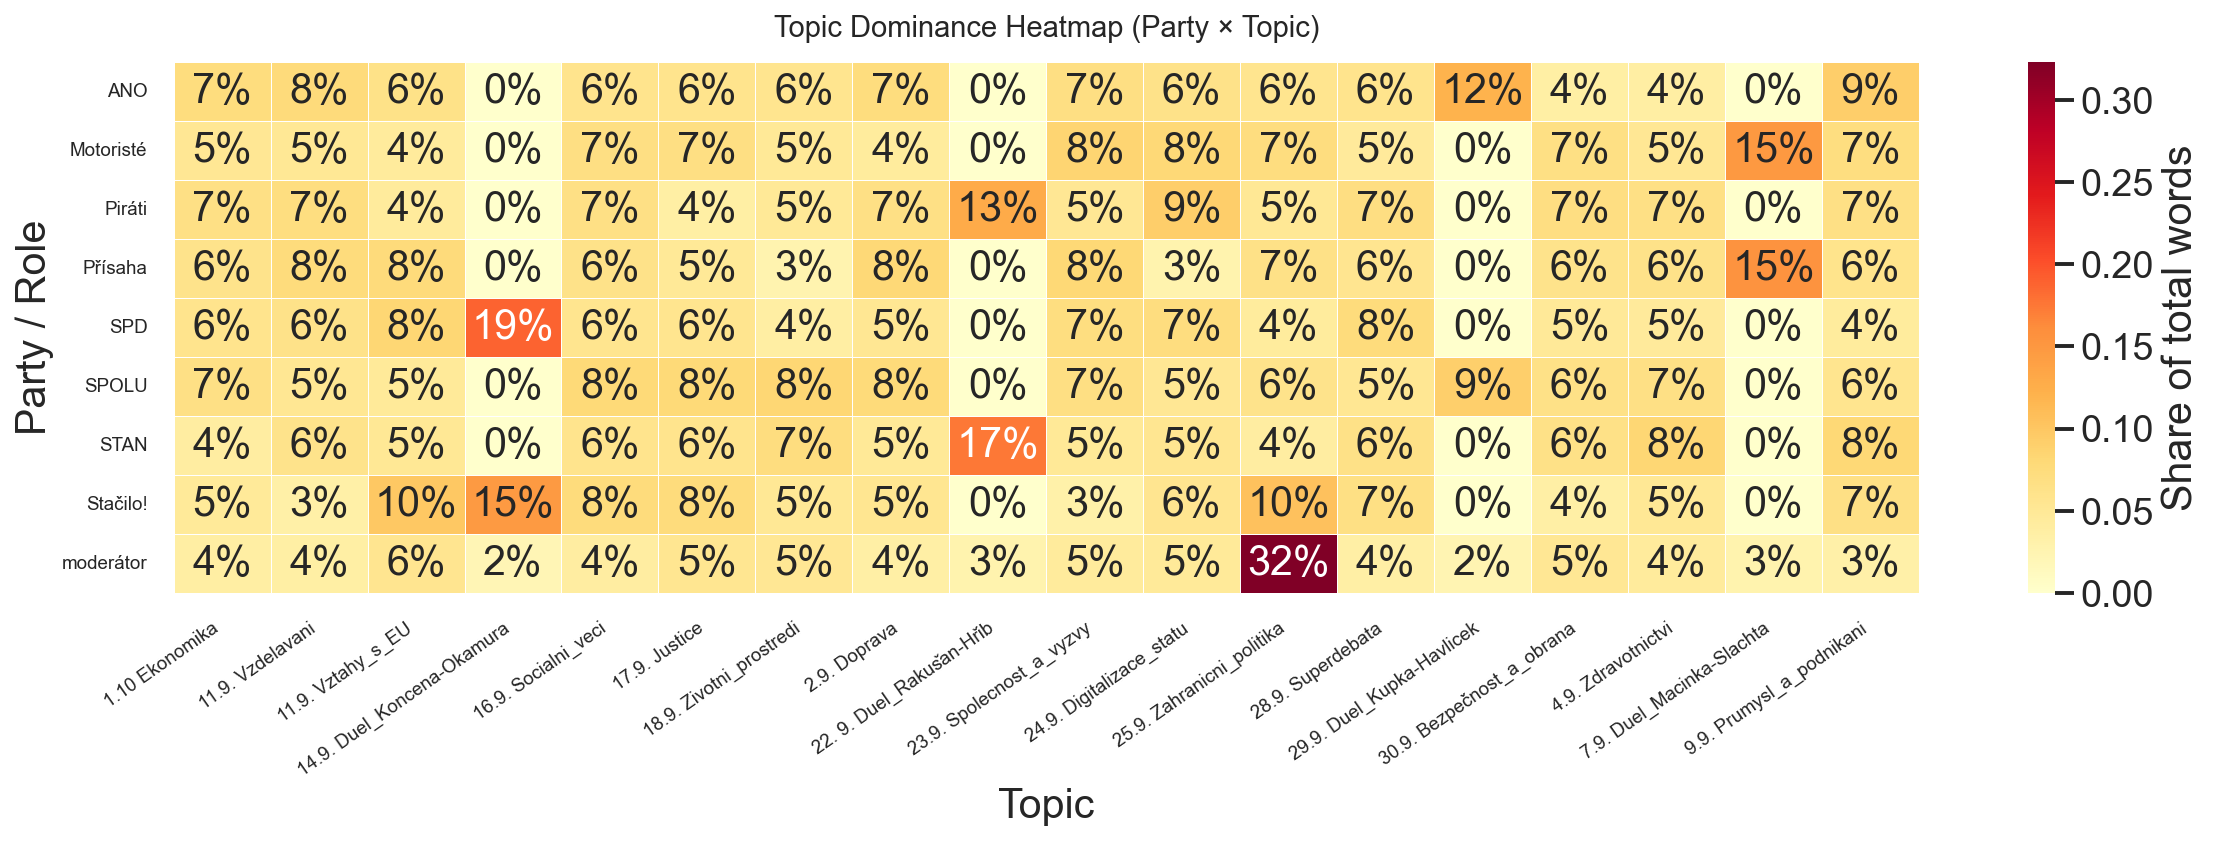
\includegraphics[width=\textwidth]{results/topic_heatmap.png}
  \caption{Heatmapa tematické dominance (Party~$\times$~Topic). Hodnoty
  udávají podíl celkového slovního rozsahu strany věnovaného danému
  tematickému bloku. Barevná škála YlOrRd — tmavší odstín indikuje
  vyšší koncentraci.}
  \label{fig:heatmap}
\end{figure}

Klíčová zjištění:

\begin{enumerate}
  \item \textbf{Superdebata jako dominantní blok.} Tematický blok
  \textit{Superdebata} (28.\,9.) koncentruje u~většiny stran 10--15\,\%
  celkového slovního rozsahu. U~strany ANO dosahuje podíl~12\,\%,
  u~SPD dokonce~15\,\%, což naznačuje strategické nasazení na tento
  formát s~vysokou sledovaností.

  \item \textbf{Duelové formáty.} Specifické duely vykazují výrazné
  koncentrace u~příslušných stran — duel \textit{Končená--Okamura}
  (14.\,9.) ukazuje zvýšenou koncentraci u~SPD (9\,\%), duel
  \textit{Rakušan--Hřib} (22.\,9.) dominuje u~STAN (17\,\%).
  Moderátor vykazuje nejvyšší koncentraci právě v~bloku
  \textit{Superdebata} (32\,\%), což odpovídá jeho řídící roli
  v~tomto rozsáhlém formátu.

  \item \textbf{Tematické preference Stačilo!} Strana Stačilo! vykazuje
  zvýšenou koncentraci v~blocích \textit{Sociální věci} (15\,\%) a~\textit{Ekonomika} (10\,\%),
  což koresponduje s~programovou orientací na sociální a~ekonomická témata.

  \item \textbf{Relativní rovnoměrnost systémových stran.} Velké
  parlamentní strany (ANO, SPOLU, Piráti) vykazují relativně rovnoměrnou
  distribuci pozornosti napříč tématy (většina hodnot v~rozmezí
  4--8\,\%), což odráží záměr pokrýt celé spektrum politických otázek.
\end{enumerate}

% ══════════════════════════════════════════════════════════════════════
\section{Diskuse}
\label{sec:diskuse}

Předložené výsledky umožňují formulovat několik obecnějších pozorování
o~povaze politického diskurzu v~české předvolební kampani~2025.

\subsection{Sémantická konvergence a~diskurzivní mainstream}

Dominantní centrální shluk v~UMAP projekci (obr.~\ref{fig:semantic_map})
naznačuje, že navzdory deklarovaným ideologickým rozdílům operují české
politické strany v~ekonomickém tématu ve~sdíleném sémantickém prostoru.
Toto zjištění je konzistentní s~teorií diskurzivního mainstreamu
(Angermuller, 2014), podle níž institucionalizovaný politický diskurz
tenduje ke~konvergenci v~základních pojmových rámcích.

Separované okrajové shluky v~sémantické mapě představují promluvy, které
se sémanticky vymykají hlavnímu proudu — mohou jít o~procedurální výroky,
emotivní prohlášení nebo stylisticky odlišné duelové formáty. Jejich
přítomnost napříč stranami potvrzuje, že sémantická odlišnost je dána
spíše komunikačním žánrem než stranickou příslušností.

\subsection{Lexikální profily jako indikátory rétorického stylu}

Kombinace TTR a~průměrné délky věty vytváří dvoudimenzionální prostor
rétorických stylů (obr.~\ref{fig:entropy}). Pozice Pirátů — s~nejdelšími
větami a~nejnižší lexikální diverzitou — indikuje diskurzivní strategii
založenou na komplexní argumentaci s~opakovaným používáním klíčových
termínů. Naopak pozice SPOLU — krátké věty, vysoká diverzita — naznačuje
komunikační styl orientovaný na heslovitost a~lexikální variabilitu.

Je třeba poznamenat, že TTR je citlivé na délku textu — delší promluvy
přirozeně vykazují nižší TTR. Maas index tuto závislost logaritmickou
transformací tlumí, přičemž pořadí stran zůstává v~obou metrikách
konzistentní, což posiluje robustnost zjištění.

\subsection{Tematické strategie a~formátové efekty}

Heatmapa tematické dominance (obr.~\ref{fig:heatmap}) odhaluje interakci
mezi stranickými preferencemi a~formátem debaty. Duelové formáty přirozeně
koncentrují slovní rozsah u~příslušných stran, zatímco Superdebata funguje
jako tematicky nejrovnoměrnější platforma. Zvýšená koncentrace menších
a~protisystémových stran na specifická témata může odrážet jak programovou
specializaci, tak strategické rozhodnutí soustředit omezený diskurzivní
prostor na vybraná témata.

\subsection{Limity studie}

Předložená analýza má několik omezení, která je třeba reflektovat:

\begin{itemize}
  \item \textbf{Tokenizace.} Použitá jazykově agnostická tokenizace
  (segmentace na mezerách) nerespektuje morfologickou strukturu češtiny.
  Lemmatizace nebo morfologická analýza by mohla poskytnout přesnější
  hodnoty lexikálních metrik.

  \item \textbf{Závislost TTR na délce.} Přestože Maas index tuto
  závislost zmírňuje, komparace stran s~výrazně odlišným počtem promluv
  (Piráti:~401 vs.\ SPOLU:~840) vyžaduje interpretační obezřetnost.

  \item \textbf{Determinismus LLM anotací.} Anotace sentimentu,
  agresivity a~rétorických rámců generované velkým jazykovým modelem
  jsou inherentně nedeterministické. Pro plnou reprodukovatelnost
  je nezbytné verzovat výstupní datový soubor.

  \item \textbf{Jednorozměrnost embeddingového modelu.}
  Použitý model \modelname{} optimalizuje sémantickou podobnost
  na úrovni parafrází; pragmatické, ironické a~konativní dimenze
  diskurzu mohou být v~embeddingu nedostatečně zachyceny.
\end{itemize}

% ══════════════════════════════════════════════════════════════════════
\section{Závěr}
\label{sec:zaver}

Předkládaná studie demonstrovala, že kvantitativní metody založené na
sentence embeddingách, redukci dimenzí a~lexikálních metrikách mohou
poskytnout systematický a~reprodukovatelný pohled na strukturu politického
diskurzu. Pipeline PDT transformuje surový textový přepis na trojici
vizualizací — sémantickou mapu, bubble chart rétorického profilu
a~heatmapu tematické dominance — které společně zachycují sémantické,
lexikální a~tematické dimenze diskurzivního prostoru.

Pro obecnou lingvistiku má navržený přístup dvojí přínos. Za prvé,
demonstroval aplikovatelnost multilinguálních sentence embeddingů na
český politický diskurz — materiál se specifickou slovní zásobou,
syntaktickou strukturou a~pragmatickými konvencemi. Za druhé, ukázal,
že kombinace kvantitativních metrik (TTR, Maas, UMAP) s~kvalitativní
interpretací grafů může generovat lingvisticky relevantní hypotézy
o~diskurzivních strategiích bez nutnosti a~priori stanovovat analytické
kategorie.

Budoucí výzkum by mohl rozšířit analýzu o~temporální dimenzi (vývoj
sémantického prostoru v~čase debaty), interakční analýzu (komu kdo
odpovídá) a~kontrastivní srovnání s~korpusy politických debat v~jiných
jazycích středoevropského prostoru.

% ══════════════════════════════════════════════════════════════════════
\section*{Literatura}
\addcontentsline{toc}{section}{Literatura}

\begin{enumerate}
  \item Angermuller, J. (2014). \textit{Poststructuralist Discourse
  Analysis: Subjectivity in Enunciative Pragmatics.} Palgrave Macmillan.

  \item Fairclough, N. (1995). \textit{Critical Discourse Analysis: The
  Critical Study of Language.} Longman.

  \item Maas, H.\,D. (1972). Über den Zusammenhang zwischen
  Wortschatzumfang und Länge eines Textes. \textit{Zeitschrift für
  Literaturwissenschaft und Linguistik,} 2(8), 73--79.

  \item McInnes, L., Healy, J., \& Melville, J. (2018). UMAP: Uniform
  Manifold Approximation and Projection for Dimension Reduction.
  \textit{arXiv preprint arXiv:1802.03426.}

  \item Reimers, N., \& Gurevych, I. (2019). Sentence-BERT: Sentence
  Embeddings using Siamese BERT-Networks. In \textit{Proceedings of the
  2019 Conference on Empirical Methods in Natural Language Processing
  (EMNLP),} 3982--3992.

  \item van Dijk, T.\,A. (2001). Multidisciplinary CDA: A Plea for
  Diversity. In R.~Wodak \& M.~Meyer (Eds.), \textit{Methods of Critical
  Discourse Analysis} (pp.~95--120). SAGE.
\end{enumerate}

\end{document}
